\documentclass[12pt,a4paper,UTF8]{article}
\usepackage{ctex} % Chinese support
\usepackage{graphicx} % Insert images
\usepackage{subfigure}
\usepackage{float}
\usepackage{listings} % Print source code
\usepackage{color} % Color support
\usepackage{booktabs} % Professional table support
\usepackage{pdflscape} % Landscape pages support in PDF
\usepackage{hyperref} % Hypertext links support for cross-referencing
\usepackage{amsmath,mathtools}
\usepackage{ulem} % strikethrough
%\usepackage{enumerate}
%\usepackage{enumitem} % indent of item

% Customize hyperref format (it's set to no special format here)
\hypersetup{hidelinks}

% Declare directories to search for graphics files for graphicx
\graphicspath{{figures/}}

% Define source code style for listings
\lstdefinestyle{verilog-style}{
	language=Verilog,
	basicstyle=\ttfamily\footnotesize,
	keywordstyle=\bfseries\color[rgb]{0, 0, 1},
	identifierstyle=\color[rgb]{0.5, 0.3, 0.1},
	stringstyle=\color[rgb]{0.6, 0.1, 0.1},
	commentstyle=\itshape\color[rgb]{0.05, 0.5, 0.05},
	backgroundcolor=\color[gray]{0.95},
	numbers=left,
	numbersep=5pt,
	numberstyle=\color[gray]{0.6},
	breaklines=true
}

\newcommand{\reporttitle}[2]{
  \LARGE\textsf{#1}\quad\underline{\makebox[12em]{#2}}
}

\newcommand{\reportinfo}[2]{
  \large\makebox[4em]{\textsf{#1}}\quad\underline{\makebox[18em]{#2}}
}

\begin{document}
\begin{titlepage}
  \centering
  \vspace*{\fill}
  {\Huge\textsf{数字电路与数字系统实验}} \\ [100pt]
  \reportinfo{实验名称}{exp01 选择器} \\ [10pt]
  \reportinfo{院系}{计算机科学与技术系} \\ [10pt]
  \reportinfo{学生姓名}{} \\ [10pt]
  \reportinfo{学号}{} \\ [10pt]
  \reportinfo{班级}{数字电路与数字系统实验1班} \\ [10pt]
  \reportinfo{邮箱}{} \\ [10pt]
  \reportinfo{实验时间}{2020 年 9 月 16 日} \\ [10pt]
  \vspace*{\fill}
\end{titlepage}
\tableofcontents
\newpage

\section{实验目的}
\begin{itemize}
  \item 学会Quartus的基本使用
  \item Verilog编程入门
  \item 设计一个2位4选1多路选择器
  \item \sout{\LaTeX从入门到入土}
  \item \sout{换一种环境和语言写bug}
  \item \sout{把已经还给老师的上学期的知识捡回来}
\end{itemize}

\section{实验原理}
多路选择器的对多路数据的选择:选择端控制输出哪一路数据

\section{实验环境/器材}
\begin{itemize}
  \item Quartus编辑器和DE10-Standard开发平台
  \item FPGA开发板
\end{itemize}

\section{程序代码或流程图}
很简单的case语句:
\begin{lstlisting}[style=verilog-style]
  module mux4to1_b2(Y, X0, X1, X2, X3, F);
	input [1:0] Y, X0, X1, X2, X3;
	output reg [1:0] F;
	
	always @ (*)
		case(Y)
			0: F = X0;
			1: F = X1;
			2: F = X2;
			3: F = X3;
			default: F = 2'b00;
		endcase
endmodule 
\end{lstlisting}

\section{实验步骤/过程}
 {
  %\renewcommand\theenumi{\Roman{enumi}}
  \newcounter{stepcnt}
  \begin{list}{(\thestepcnt)}{\usecounter{stepcnt}} %\setlength{\itemindent}{1em}
    \item 首先用DE10\_Standard\_SystemBuilder创建工程,
          只需要勾选LED和Switch即可,这样可以自动分配引脚
    \item 接着当然是简单写一写代码
    \item 写完之后进行编译,然后用RTL Viewer看一下内部实现的结构
          \begin{figure}[H]
            \centering
            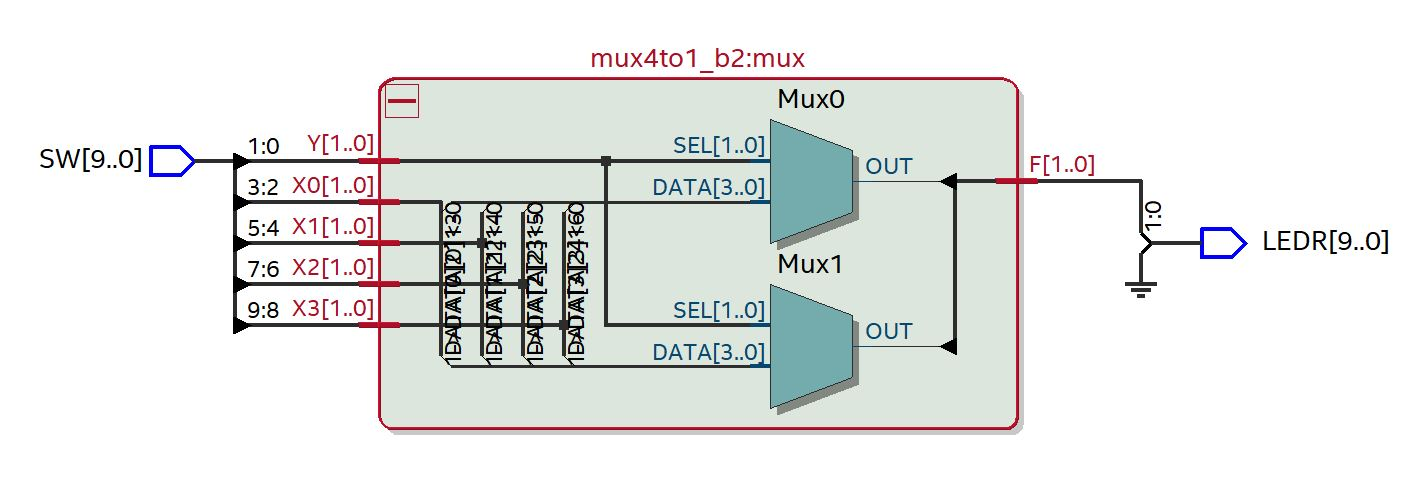
\includegraphics[width=0.8\textwidth]{mux_RTL.JPG}
            \caption{mux4to1\_b2的原理图}
            \label{mux_RTL}
          \end{figure}

    \item 然后编写测试代码,测试完后用FPGA验证一下就完成了(详见下一条目)
  \end{list}
 }

\section{测试方法}
\begin{description}
  \item[\hspace{2em}测试代码] \hspace*{\fill}
        \begin{itemize}
          \item 分别给X0$\sim$X3赋值00$\sim$11,Y初始化为00
          \item 然后每隔10个时间单位将Y加1,直到Y的值为11
          \item 对照仿真波形图分析验证
        \end{itemize}
  \item [\hspace{2em}硬件验证] \hspace*{\fill}
        \begin{itemize}
          \item 将.sof文件写入FPGA,然后拨动开关观察指示灯输出进行验证
        \end{itemize}
\end{description}

\section{实验结果}
\begin{itemize}
  \item 运行仿真结果如下图。绿线中的最下面两条对应LED输出,
        绿线中从下向上数第三第四条对应选择输入端Y,分析可知输出满足要求
        \begin{figure}[H]
          \centering
          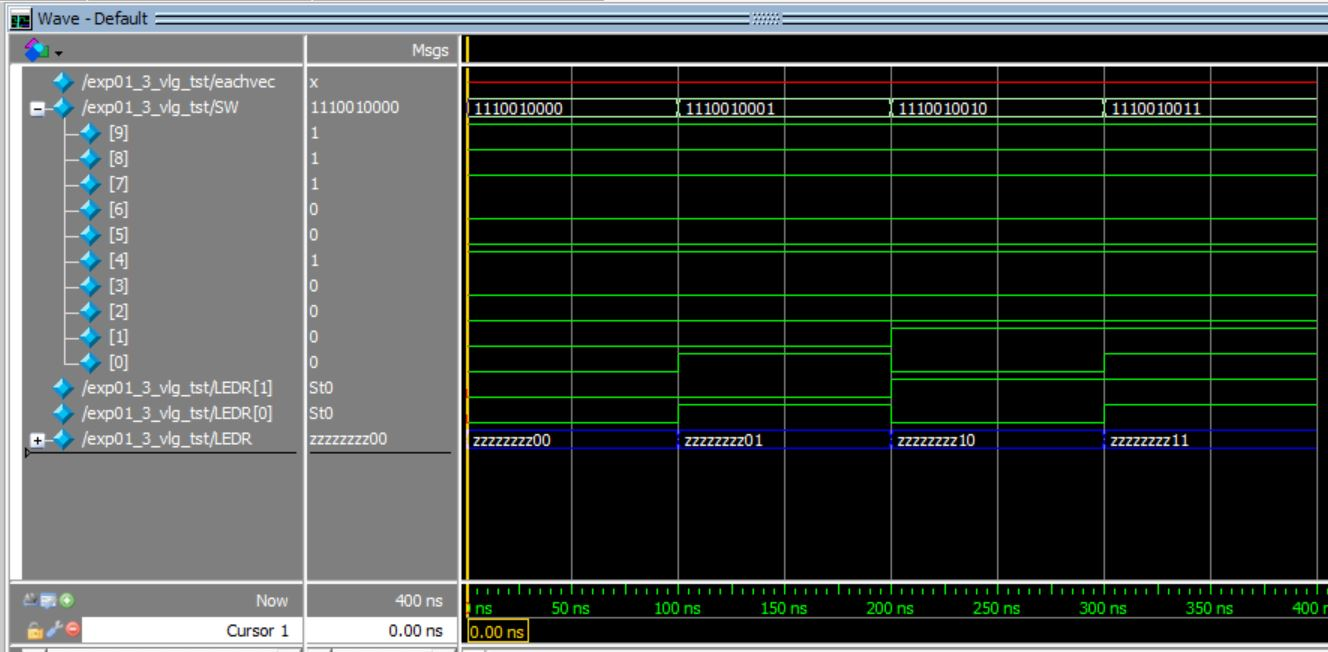
\includegraphics[width=0.8\textwidth]{mux_sim.JPG}
          \caption{运行仿真结果}
          \label{mux_sim}
        \end{figure}
  \item 写入FPGA之后对每种选择和数据输入都进行了验证,均满足要求
        \begin{figure}[H]
          \centering
          \subfigure[Y=10, X2=11]{
            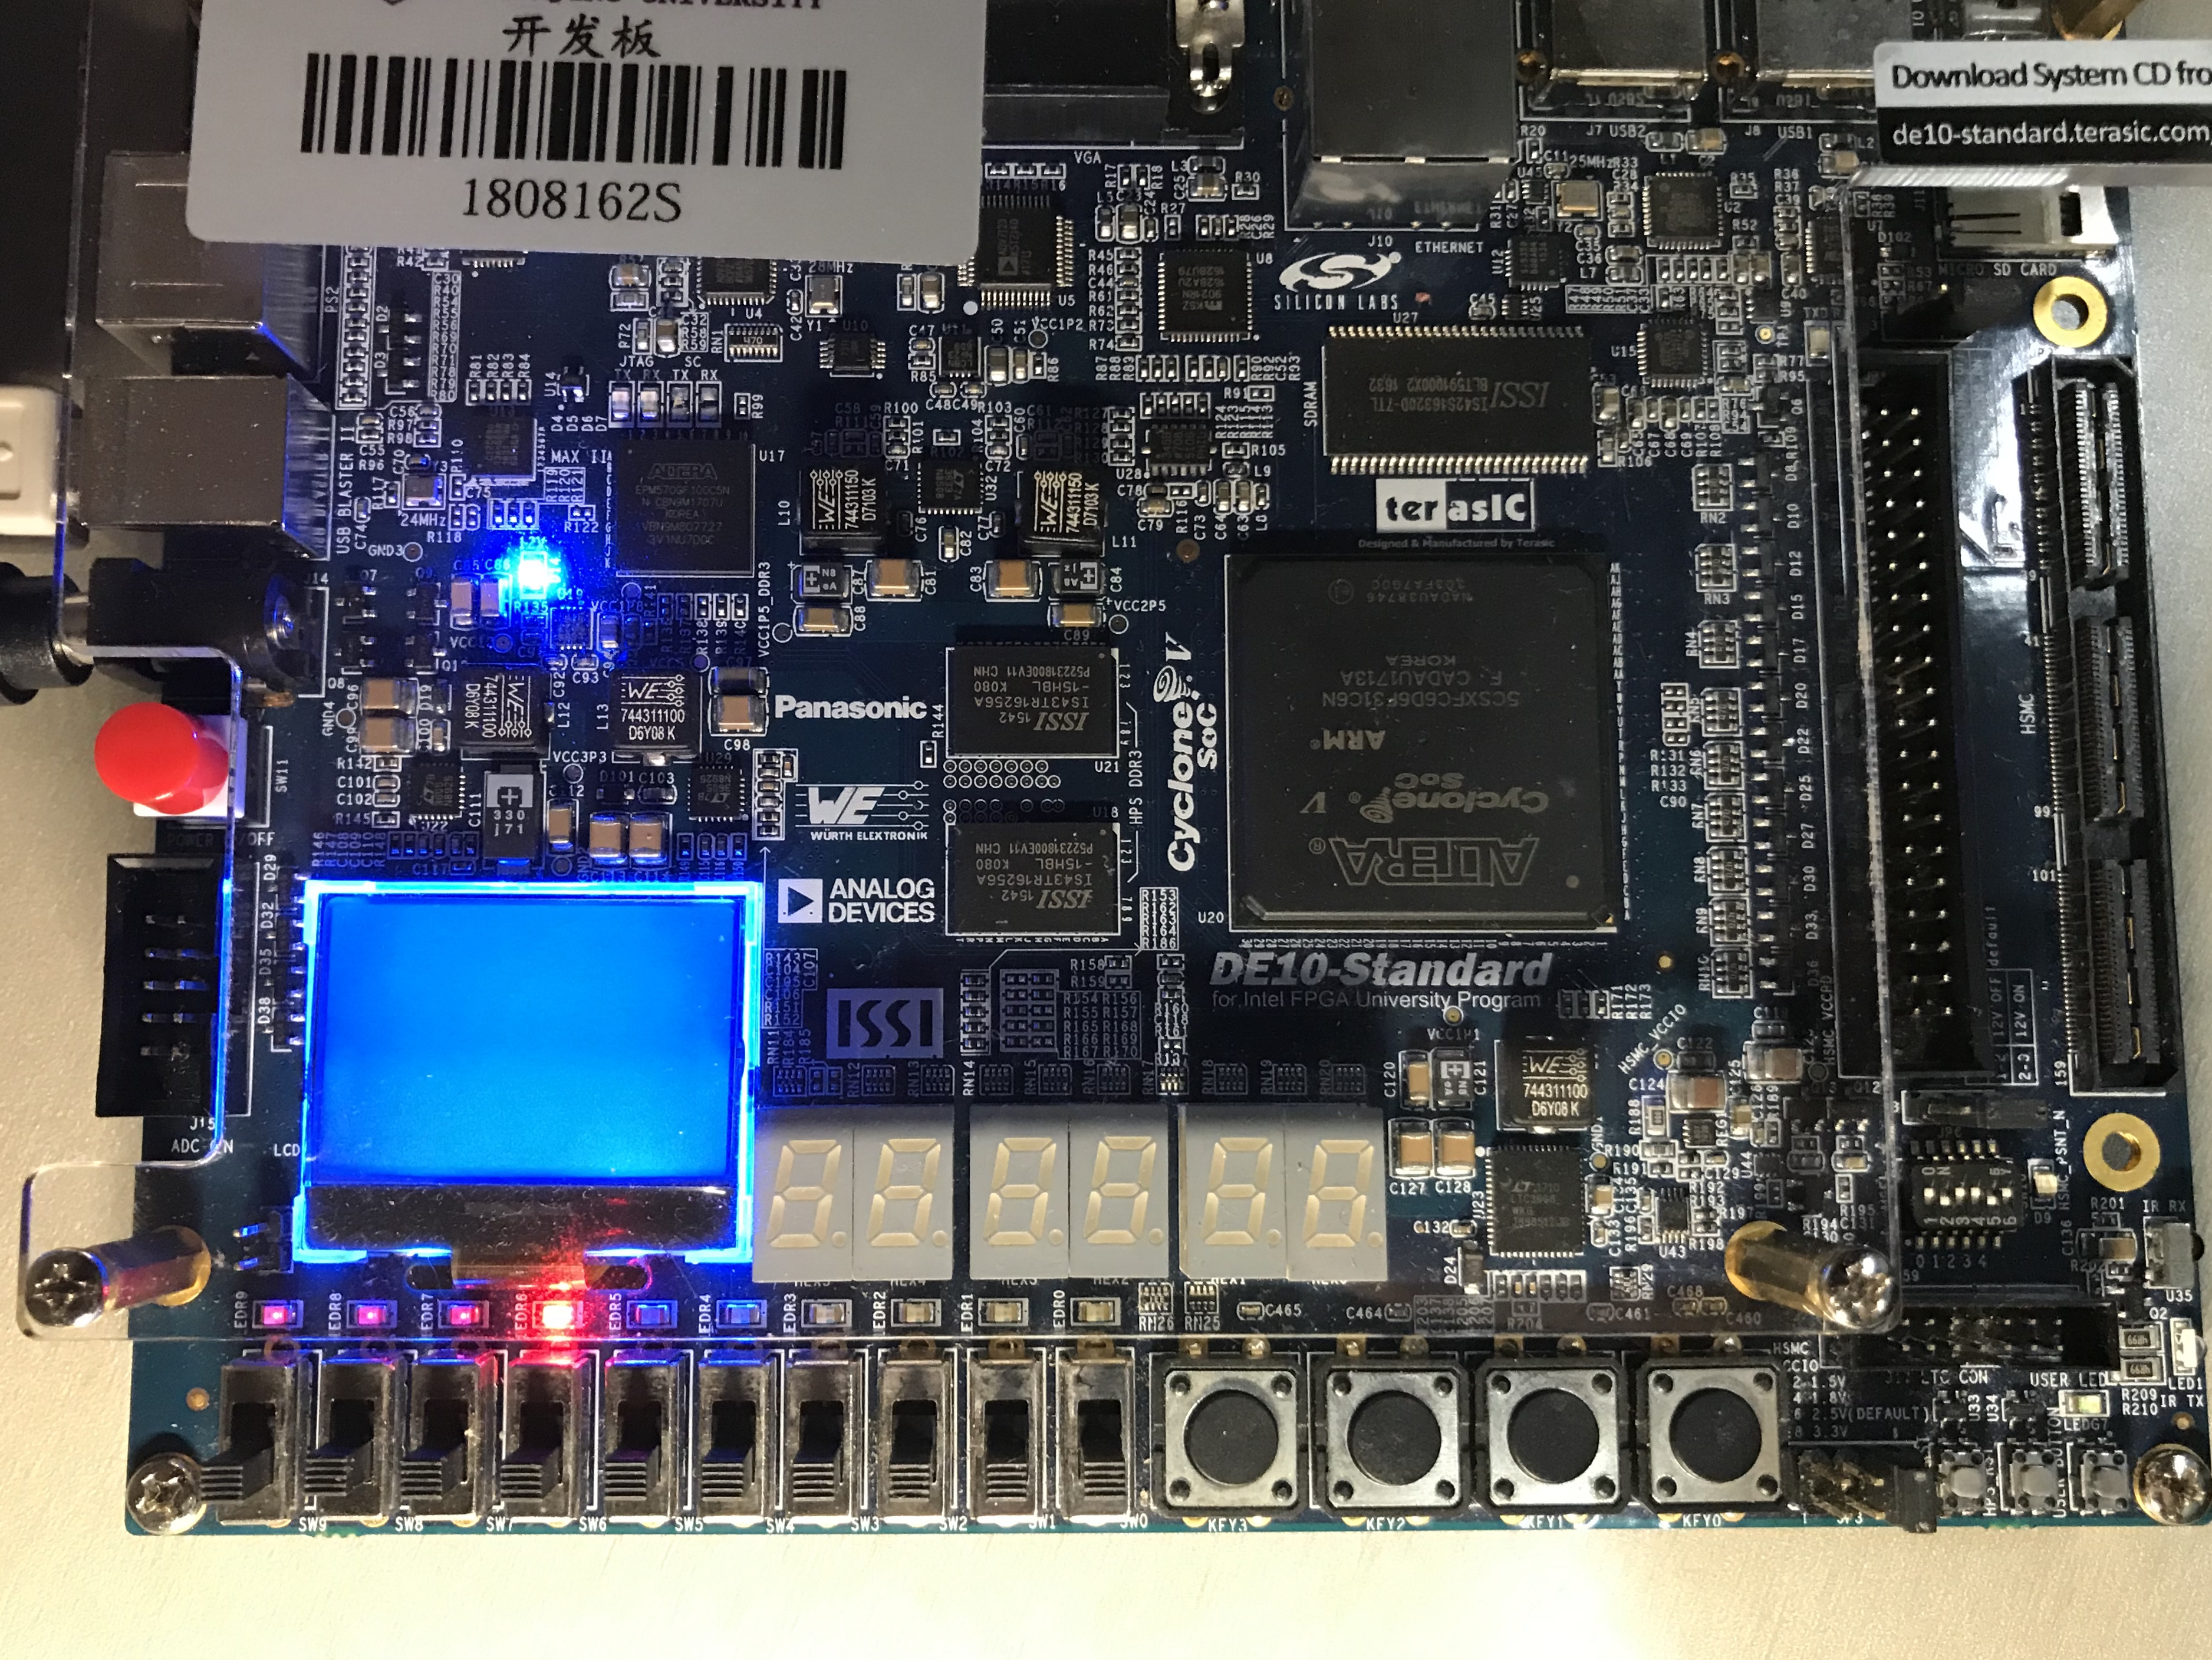
\includegraphics[width=0.45\textwidth]{fpga1.JPG}
          }
          \subfigure[Y=00, X0=11]{
            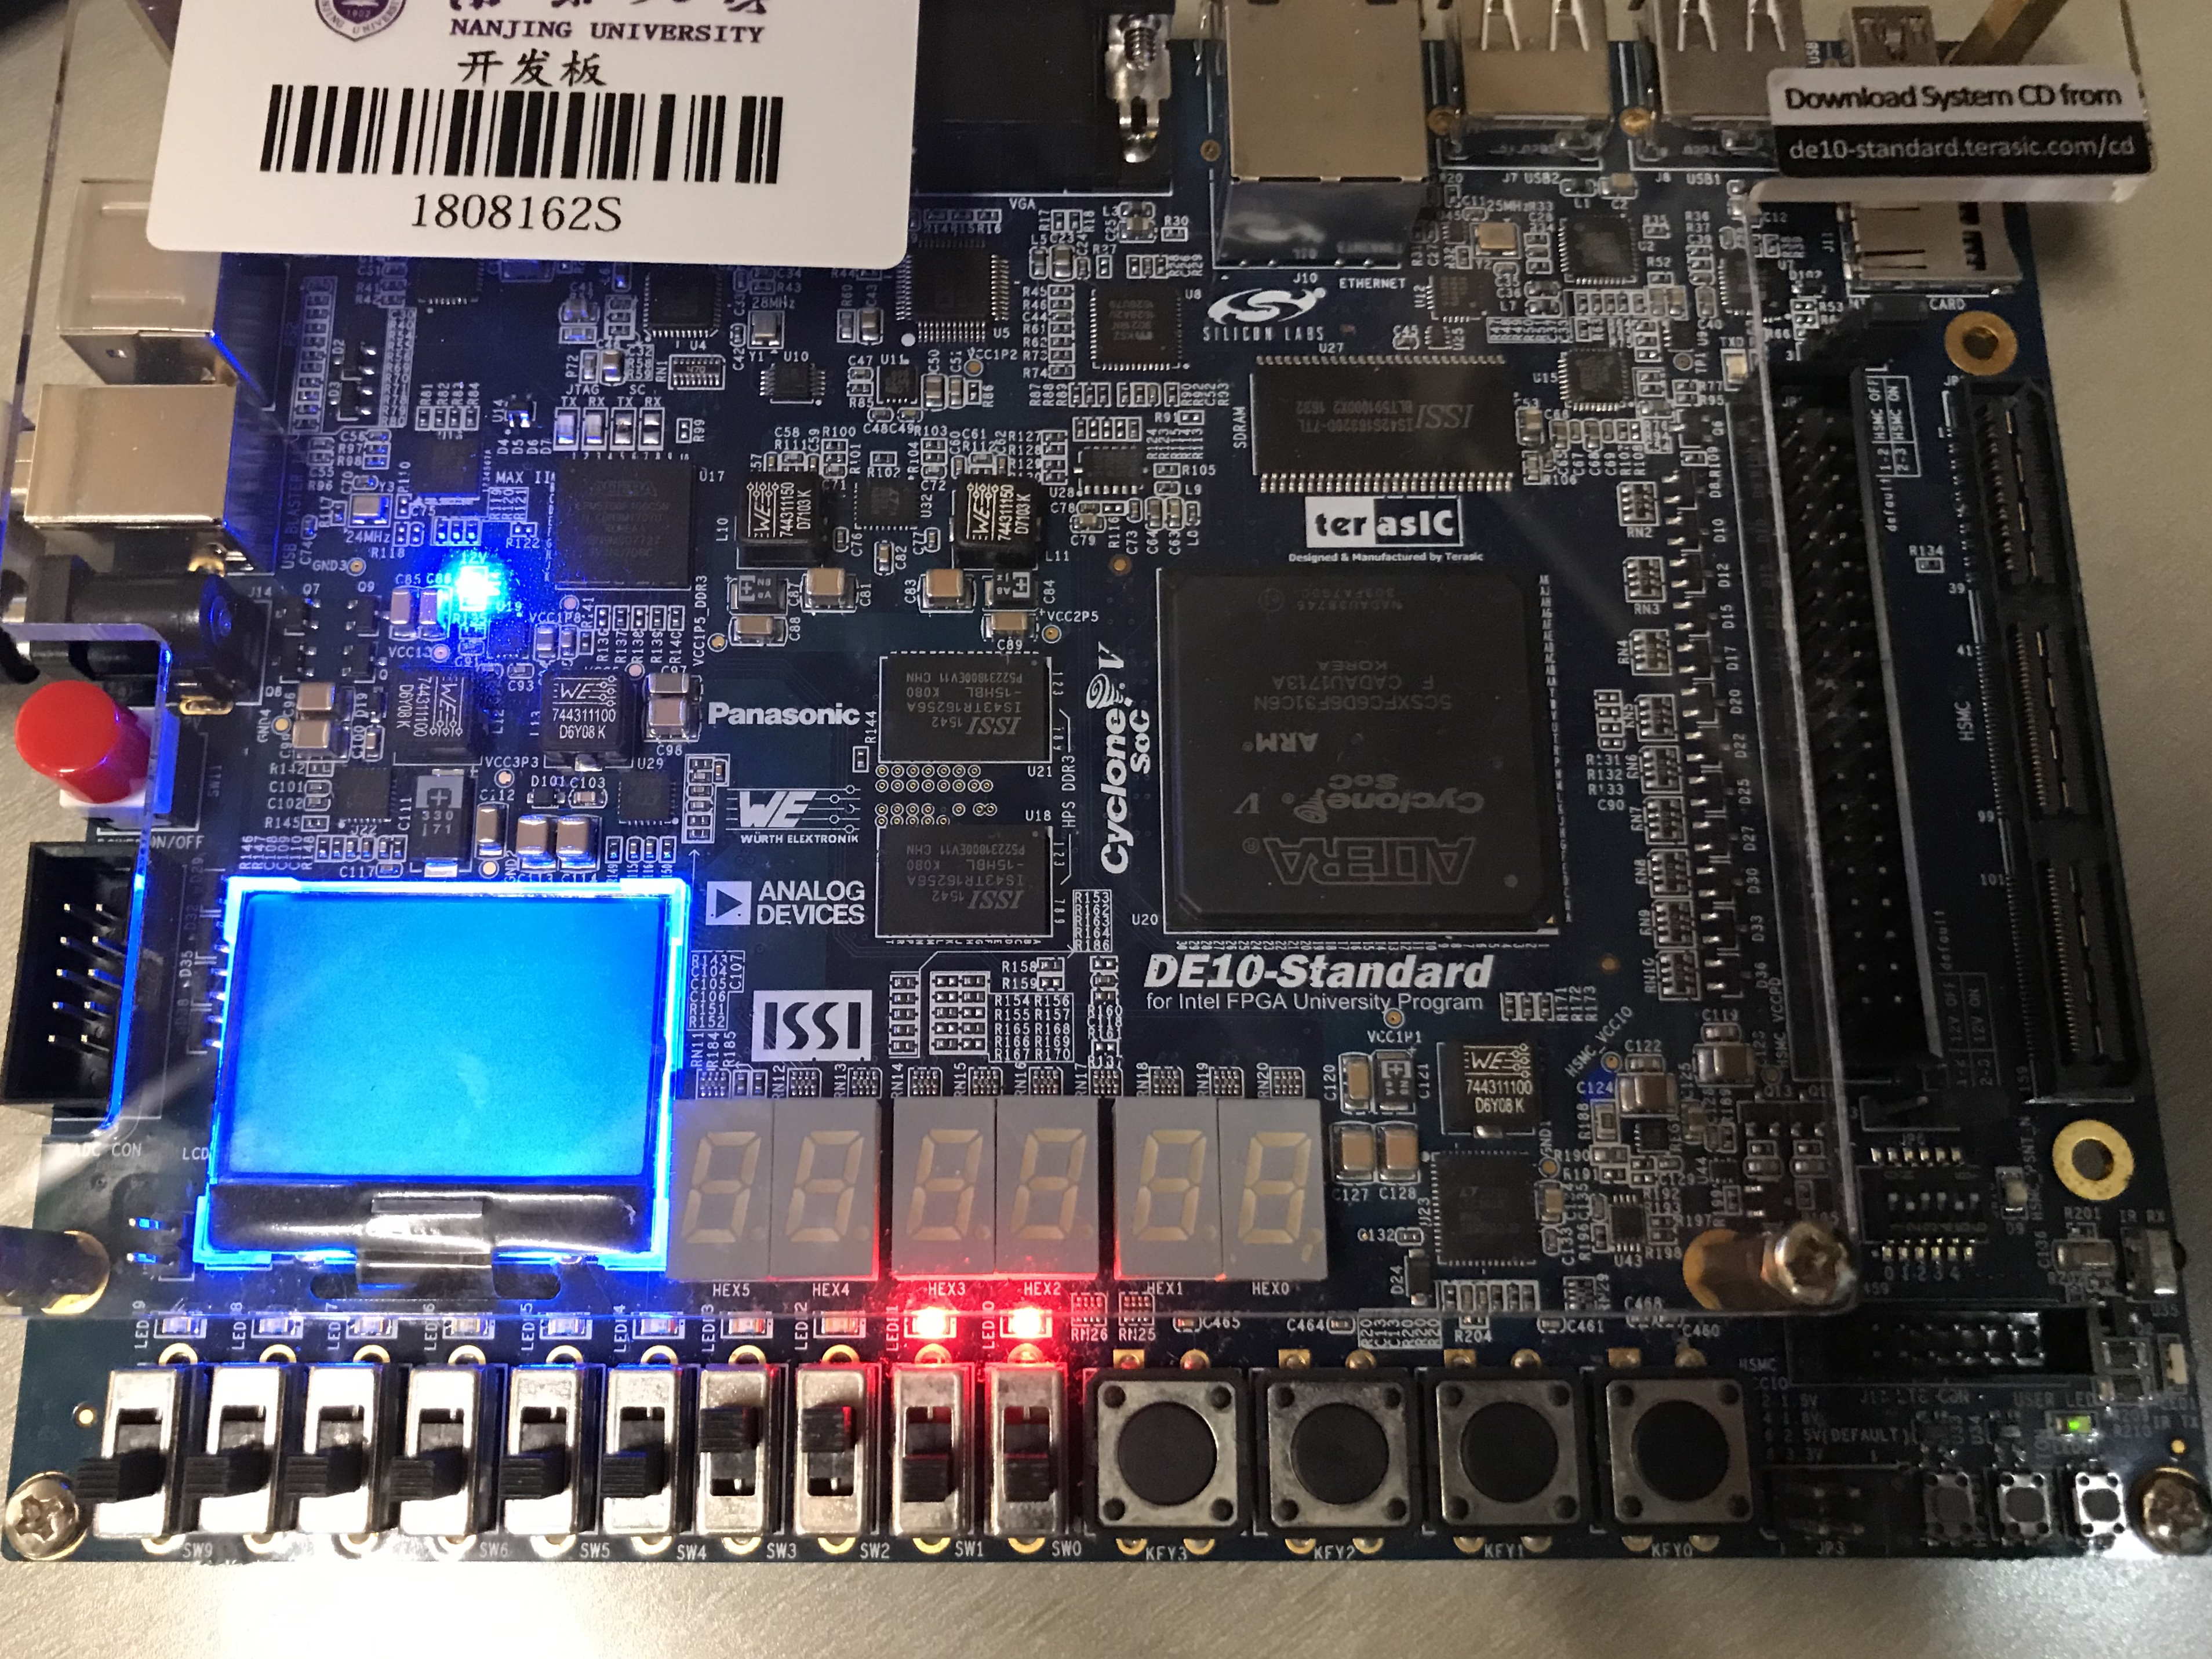
\includegraphics[width=0.45\textwidth]{fpga2.JPG}
          }
          \caption{其中两种情况的截图}
          \label{fpga}
        \end{figure}
\end{itemize}

\section{遇到的问题及解决办法}
\begin{itemize}
  \item 老师给出的安装教程及使用教程十分详细,并没有遇到什么大问题
  \item 唯一遇到的一个小问题是,因为要让工程自动分配引脚,所以用\linebreak[4]
        DE10\_Standard\_SystemBuilder创建工程,但是用这种方法
        创建出来的工程文件夹中没有simulation文件夹和output\_files文件夹。
        解决方法是Assignments$\rightarrow$settings$\rightarrow$
        Simulation$\rightarrow$Tool name项选择ModelSim-Altera,
        这样之后再运行,工程文件夹中就会出现simulation文件夹了。
        然后就可以按照视频里的步骤继续进行运行仿真的操作了。
  \item 关于output\_files文件夹的问题还没有找到解决方案,但是因为
        这对实验没有太大的影响,所以暂时先搁置(如果助教老师能告诉我
        解决方案那就太感谢了)
  \item \sout{第一次写\LaTeX遇到了一万个问题但是这里太窄了写不下}
\end{itemize}

\section{得到的启示}
\begin{itemize}
  \item case的default项所赋的值应该是0,因为当输入为其他情况时
        LED灯不会亮,输出应为0
  \item 在测试实验中,可以通过给每个数据输入赋不同的值,
        然后根据选择输入判断输出是否满足要求
  \item \sout{\LaTeX排版好好看啊呜呜呜}
\end{itemize}

\section{意见和建议}
\begin{itemize}
  \item 希望助教老师能介绍一下这个问题的解决办法(``遇到的问题''条目中所描述):
        用DE10\_Standard\_SystemBuilder创建工程后如何生成\linebreak[4]
        output\_files文件夹,以及如何让.sof等文件生成在该文件夹中
\end{itemize}

\end{document}